% Options for packages loaded elsewhere
\PassOptionsToPackage{unicode}{hyperref}
\PassOptionsToPackage{hyphens}{url}
%
\documentclass[
]{book}
\usepackage{amsmath,amssymb}
\usepackage{lmodern}
\usepackage{ifxetex,ifluatex}
\ifnum 0\ifxetex 1\fi\ifluatex 1\fi=0 % if pdftex
  \usepackage[T1]{fontenc}
  \usepackage[utf8]{inputenc}
  \usepackage{textcomp} % provide euro and other symbols
\else % if luatex or xetex
  \usepackage{unicode-math}
  \defaultfontfeatures{Scale=MatchLowercase}
  \defaultfontfeatures[\rmfamily]{Ligatures=TeX,Scale=1}
\fi
% Use upquote if available, for straight quotes in verbatim environments
\IfFileExists{upquote.sty}{\usepackage{upquote}}{}
\IfFileExists{microtype.sty}{% use microtype if available
  \usepackage[]{microtype}
  \UseMicrotypeSet[protrusion]{basicmath} % disable protrusion for tt fonts
}{}
\makeatletter
\@ifundefined{KOMAClassName}{% if non-KOMA class
  \IfFileExists{parskip.sty}{%
    \usepackage{parskip}
  }{% else
    \setlength{\parindent}{0pt}
    \setlength{\parskip}{6pt plus 2pt minus 1pt}}
}{% if KOMA class
  \KOMAoptions{parskip=half}}
\makeatother
\usepackage{xcolor}
\IfFileExists{xurl.sty}{\usepackage{xurl}}{} % add URL line breaks if available
\IfFileExists{bookmark.sty}{\usepackage{bookmark}}{\usepackage{hyperref}}
\hypersetup{
  pdftitle={Eagle I.O Consultant Manual},
  pdfauthor={Eagle I.O},
  hidelinks,
  pdfcreator={LaTeX via pandoc}}
\urlstyle{same} % disable monospaced font for URLs
\usepackage{longtable,booktabs,array}
\usepackage{calc} % for calculating minipage widths
% Correct order of tables after \paragraph or \subparagraph
\usepackage{etoolbox}
\makeatletter
\patchcmd\longtable{\par}{\if@noskipsec\mbox{}\fi\par}{}{}
\makeatother
% Allow footnotes in longtable head/foot
\IfFileExists{footnotehyper.sty}{\usepackage{footnotehyper}}{\usepackage{footnote}}
\makesavenoteenv{longtable}
\usepackage{graphicx}
\makeatletter
\def\maxwidth{\ifdim\Gin@nat@width>\linewidth\linewidth\else\Gin@nat@width\fi}
\def\maxheight{\ifdim\Gin@nat@height>\textheight\textheight\else\Gin@nat@height\fi}
\makeatother
% Scale images if necessary, so that they will not overflow the page
% margins by default, and it is still possible to overwrite the defaults
% using explicit options in \includegraphics[width, height, ...]{}
\setkeys{Gin}{width=\maxwidth,height=\maxheight,keepaspectratio}
% Set default figure placement to htbp
\makeatletter
\def\fps@figure{htbp}
\makeatother
\setlength{\emergencystretch}{3em} % prevent overfull lines
\providecommand{\tightlist}{%
  \setlength{\itemsep}{0pt}\setlength{\parskip}{0pt}}
\setcounter{secnumdepth}{5}
\usepackage{booktabs}
\usepackage{booktabs}
\usepackage{longtable}
\usepackage{array}
\usepackage{multirow}
\usepackage{wrapfig}
\usepackage{float}
\usepackage{colortbl}
\usepackage{pdflscape}
\usepackage{tabu}
\usepackage{threeparttable}
\usepackage{threeparttablex}
\usepackage[normalem]{ulem}
\usepackage{makecell}
\usepackage{xcolor}
\ifluatex
  \usepackage{selnolig}  % disable illegal ligatures
\fi
\usepackage[]{natbib}
\bibliographystyle{apalike}

\title{Eagle I.O Consultant Manual}
\author{Eagle I.O}
\date{Most recently updated Wednesday July 07 2021 4:51:59 PM Eastern}

\begin{document}
\maketitle

{
\setcounter{tocdepth}{4}
\tableofcontents
}
\hypertarget{homepage}{%
\chapter*{Homepage}\label{homepage}}
\addcontentsline{toc}{chapter}{Homepage}


\includegraphics{images/eagleio dot.jpg}

This is the student consultant handbook for members of Eagle I.O. Herein lie expectations, responsibilities, and strategy to keep Eagle I.O sustainable with future \href{https://www.montclair.edu/psychology/graduate-programs/industrial-organizational-psychology/}{Montclair State University I/O Psychology} cohorts\ldots{}

\hypertarget{introduction}{%
\chapter{Introduction}\label{introduction}}

\includegraphics{images/intro.PNG}

\textbf{About us}:

We are a \href{https://eagle-io.weebly.com/}{student-led consulting group} within the Industrial/Organizational Psychology program at \href{https://www.montclair.edu/psychology/graduate-programs/industrial-organizational-psychology/}{Montclair State University}, founded in 2019. We look at ourselves as hard-working, driven students who wish to strengthen MSU's I/O Psychology program, as well as learn outside of the classroom to build upon our skills and knowledge. We pride ourselves with strong involvement in local and national I/O groups, namely \href{https://metroapppsych.com/}{METRO} and \href{https://siop.org}{SIOP}.

\textbf{Our mission}:

Eagle I.O is established to provide students practical and applied learning experiences to develop skills aligned with their personal and professional goals. The group collaborates to execute a variety of I/O internal and external projects. Eagle I.O strives to prepare students to succeed after integrating into the workforce post-graduation.

\textbf{What we do}:

We are responsible for executing various projects. Our main project is developing an Engagement survey, which we wish to distribute to external organizations. We also run a mentorship program within the MSU I/O program, where we train most of the 2nd year graduate students to guide the new students into becoming successful students themselves. Additionally, we host a variety of events, such as new student orientation, networking opportunities, and casual hangouts.

\hypertarget{duties}{%
\chapter{Membership}\label{duties}}


\includegraphics{images/duty.jpg}

All members are expected to participate approximately 8 hours per week, although there is quite a bit of variability around this number depending on current projects. Members are furthermore expected to be reasonably available over Winter and Summer breaks.

\hypertarget{current-members}{%
\section{Current members\ldots{}}\label{current-members}}

\ldots need to attend all Eagle I.O meetings (unless there is a legitimate reason for absence), maintain a GPA greater than 3.5, actively participate both within the group and with the products, and lead at least one project within their first 2 semesters of membership.

\hypertarget{new-members}{%
\section{New members\ldots{}}\label{new-members}}

\ldots need to attend all meetings \protect\hyperlink{timetable}{in the latter half of the Spring semester}, maintain a GPA greater than 3.5, engage in OCB's, be responsive to professors, and actively contribute to the program culture at MSU.

\hypertarget{late}{%
\subsection[Opportunity for late admission ]{\texorpdfstring{Opportunity for late admission \footnote{If there is an interested student who is unable to join due to the group being ``full'' (or due to personal time constraints), they are permitted to join any mini-team within Eagle I.O.}}{Opportunity for late admission }}\label{late}}

This section outlines the procedure to follow if a student missed the recruitment window, but has indicated an interest to ``join late''

Currently, Eagle I.O is limited to a maximum 10 student member cap.

If the current occupancy of Eagle I.O is less than 10, then there is a list of minimum requirements to be met prior to being accepted into Eagle I.O:

\begin{itemize}
\tightlist
\item
  1 semester of enrollment within the MSU I/O Psychology program
\item
  3.8 GPA
\item
  At least 1 semester remaining in the program
\item
  An expressed interest
\end{itemize}

Under special circumstances (as discussed by all members of Eagle I.O) students may be allowed to join \protect\hyperlink{late}{outside the period of recruitment}. The decision for membership must be discussed by all current members of Eagle I.O and be unanimous.

Criteria

\begin{itemize}
\tightlist
\item
  Current GPA 3.5 or higher
\item
  Organizational Citizenship Behavior (OCBs) - such as presence at events or hangouts
\item
  Involvement in the membership program
\item
  Completed at least 1 semester of classes in the program (Masters' or Ph.D.)
\end{itemize}

\hypertarget{eagle-i.o-expectations-all-members}{%
\section{Eagle I.O expectations (all members)}\label{eagle-i.o-expectations-all-members}}

Regardless of whether a new or continuing member, all student consultants are held to the following expectations:

\begin{itemize}
\tightlist
\item
  Coordinate and attend Fall semester orientation session
\item
  Attend mandatory bi-weekly meetings during Fall and Spring semesters

  \begin{itemize}
  \tightlist
  \item
    Stay active and engaged during summer
  \end{itemize}
\item
  Be a professional ambassador (aligned with: 1) Eagle, 2) MSU, and 3) the larger discipline of I-O Psychology)

  \begin{itemize}
  \tightlist
  \item
    Attend Eagle I.O events (METRO, social meetings, mentor meetings)
  \end{itemize}
\item
  Contribute to at least one Eagle I.O project (mentorship program, survey developments)
\item
  Annually review (and update if warranted) the Mentorship and Consultant manuals
\item
  Participate as a mentor in the Mentorship program
\item
  Meet the specific \protect\hyperlink{roles}{role requirements}

  \begin{itemize}
  \tightlist
  \item
    Successfully execute the responsibilities of the assigned role
  \end{itemize}
\end{itemize}

\hypertarget{eagle-i.o-ksas-all-members}{%
\section{Eagle I.O KSA's (all members)}\label{eagle-i.o-ksas-all-members}}

Regardless of whether a new or continuing member, the expectations are that student consultants will be reasonably characterized as:

\begin{itemize}
\tightlist
\item
  Ability to work in a team-based environment
\item
  Be receptive to group members' opinions and suggestions
\item
  Take initiative to develop current and future projects
\item
  Ability to communicate verbally and in writing
\item
  Critical thinking
\item
  Self-motivation
\item
  Being flexible
\item
  Determination and persistence
\item
  Ability to organize
\end{itemize}

\hypertarget{conflict}{%
\section{Conflict}\label{conflict}}

Eagle I.O members are expected to behave maturely and engage with other members in a respectful and understanding manner. Should arguments and/or disagreements occur regarding decision-making, the faculty advisor has the final say.

If continuous conflict originates from a singular member against the rest of the group, that member will be placed on probation for one semester at the discretion of the faculty advisor.

Once the member returns from their probation, if they continue to engage in aggressive and/or disrespectful behaviors towards the other members, they will be executed.

\hypertarget{governance}{%
\chapter{Governance}\label{governance}}

\includegraphics{images/governance.png}

\hypertarget{meetings}{%
\section{Meetings}\label{meetings}}

Regarding time expectations of Eagle I.O members:

\begin{itemize}
\tightlist
\item
  Meetings are mandatory - there is one excused absence per academic semester (Fall and Spring)

  \begin{itemize}
  \tightlist
  \item
    If you miss \emph{more than one} meeting, and cannot call or make other arrangements for your virtual attendence, you will be put on probation (1 semester term)
  \item
    If you miss another meeting while on probation you will be expelled from Eagle I.O and fed to \textbf{Sir pSyCaDeLiCaT} in an agonizingly painful yet exceedingly beautiful ceremony
  \end{itemize}
\end{itemize}

\hypertarget{consultant-development-plan}{%
\section{\texorpdfstring{\href{https://docs.google.com/document/d/13OhBJgO4Lr40uA9s3tLBTm17TNRrQa-NJnfTIbSGmT4/edit?usp=sharing}{Consultant development plan}}{Consultant development plan}}\label{consultant-development-plan}}

Each consultant, in collaboration with one of the faculty advisors, will complete an individual development plan that is specific to their individualized developmental goals within Eagle I.O. A template plan is available \href{https://docs.google.com/document/d/13OhBJgO4Lr40uA9s3tLBTm17TNRrQa-NJnfTIbSGmT4/edit?usp=sharing}{here}. Example skills to consider developing within Eagle I.O functions include professional, I/O content-domain specific, and/or technical (\texttt{R}-oriented) skills.

The intent is for each student member to meet with a Faculty Advisor in \emph{April of their 1st year of Eagle I.O participation} to determine at least one personal consultant goal that will be accomplished prior to graduation from the MSU I/O program. Each student is also expected to meet with a Faculty Advisor toward the end of the Fall semester (of their second semester of Eagle I.O participation) to monitor goal progress.

\hypertarget{roles}{%
\section{Structure}\label{roles}}

As of Summer 2021, the formal roles of Eagle I.O are:

\begin{itemize}
\tightlist
\item
  Faculty roles:

  \begin{itemize}
  \tightlist
  \item
    Advisor (primary)
  \item
    Advisor (mentorship)
  \end{itemize}
\item
  Student roles:

  \begin{itemize}
  \tightlist
  \item
    Governance officer
  \item
    Engagement officer
  \item
    Social media and website coordinator
  \item
    Student mentorship coordinator
  \item
    Alumni mentorship coordinator\\
  \item
    Event coordinator
  \item
    Parliamentarian
  \item
    R mentor
  \item
    Executive consultant
  \end{itemize}
\end{itemize}

The following chart is somewhat showing off interactive graphs generated by \texttt{R}, but if you hover over a role, you will also get a sense of interdependencies (e.g., estimates of which other roles are most intertwined with the role of focus). Directionality is implied in the figure, although the actual execution of all interactions is intended to be bi-directional.

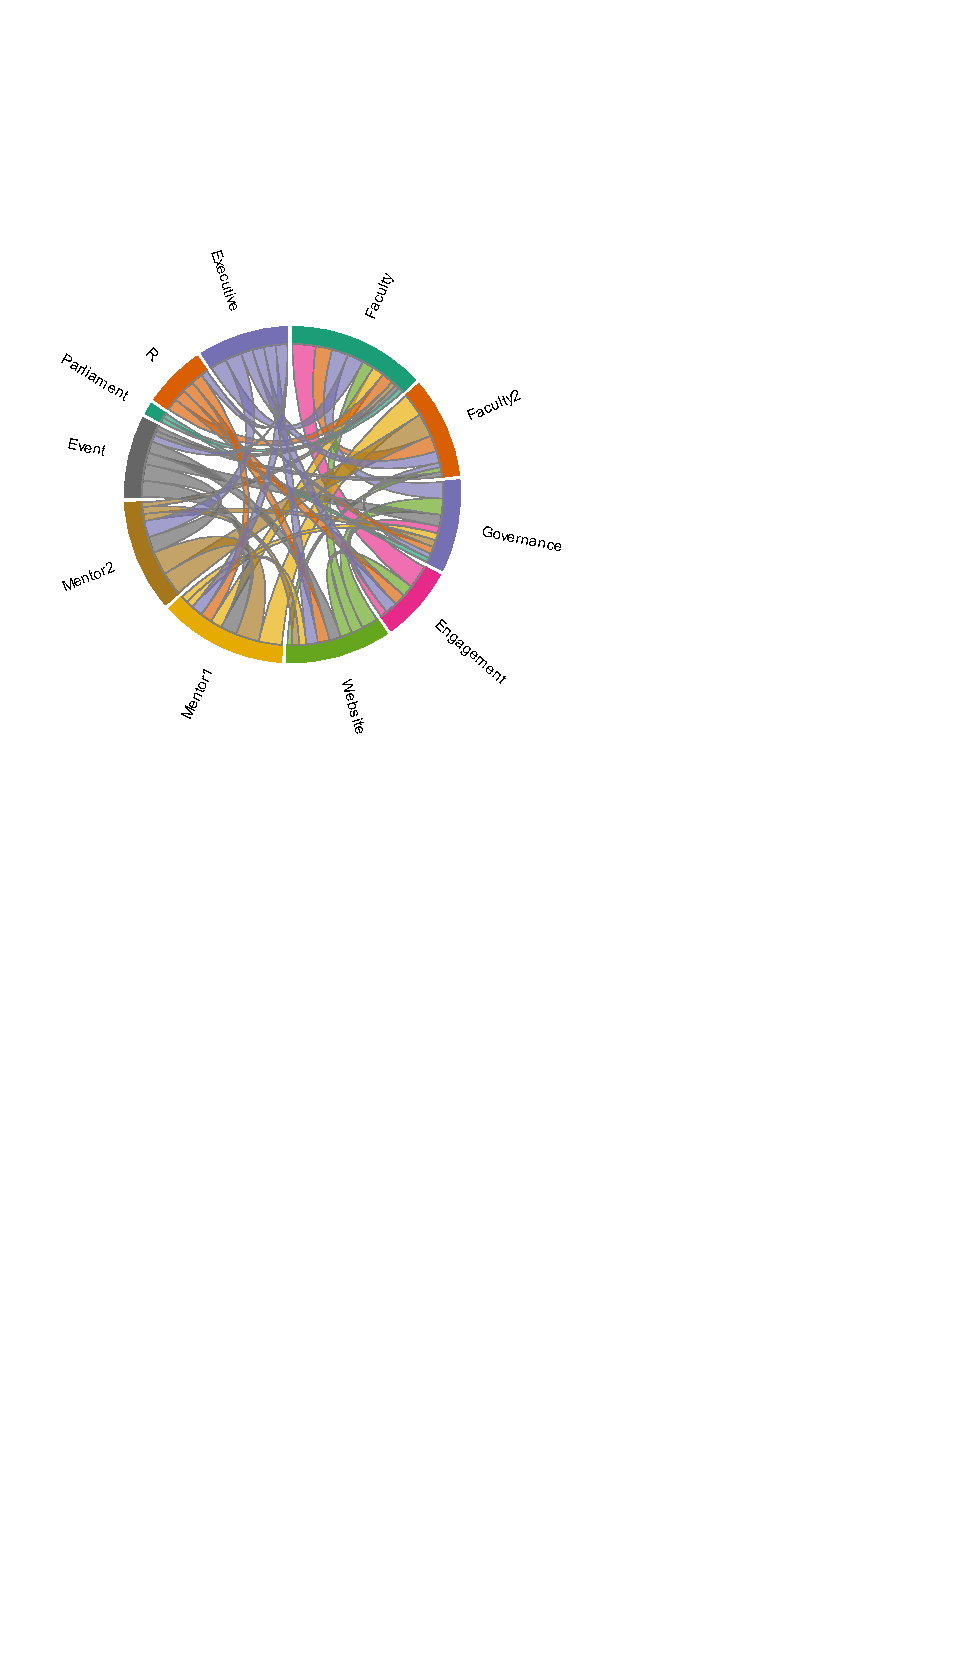
\includegraphics{manual_files/figure-latex/FunkyInteractiveChart-1.pdf}

Additional roles can be assigned on an as needed (e.g., project-by-project) basis. The primary responsibilities of these position holders are presented below. Note that role holders are responsible for the accomplishment of their assigned duties, but they are expected to execute tasks within teams (e.g., they are not expected to ``do all of the work'' on their own).

\textbf{Faculty Advisor}:

\begin{itemize}
\tightlist
\item
  Long-term visioning (5-year plan)
\item
  Annual goal-setting and monitoring (projects, clients, research)
\item
  Budgeting and staffing
\end{itemize}

\textbf{Faculty Mentorship Coordinator}:

\begin{itemize}
\tightlist
\item
  Establish and maintain alumni contact list\\
\item
  Integrate alumni and current student populations\\
\item
  Assist Mentorship Coordinator with program management
\end{itemize}

\textbf{Governance Officer}:

\begin{itemize}
\tightlist
\item
  Acts as project manager using Trello to track each member's progress within their roles, members' involvement in projects, and project updates
\item
  Uses Excel to organize members' involvement in projects
\item
  Ensures group dynamic is working
\item
  Leads membership recruitment and selection process\\
\item
  Leads sustainability change management process once a year
\end{itemize}

\textbf{Event Coordinator}:

\begin{itemize}
\tightlist
\item
  Updates all contact lists for events (incoming students, current students, alumni, and faculty)
\item
  Creates and emails invitations for events
\item
  Obtains graduation stoles for graduating members of Eagle I.O "Coordinate logistics of annual events (orientation, mid-year soiree, SIOP, etc)
\item
  GroupMe coordinator
\end{itemize}

\textbf{Engagement Coordinator}:

\begin{itemize}
\tightlist
\item
  Administration, scoring, and reporting
\item
  Norms development and maintenance
\item
  Ongoing validation studies and technical report generation\\
\item
  Delegating project-related tasks to others
\end{itemize}

\textbf{Student Mentorship Coordinator}:

\begin{itemize}
\tightlist
\item
  Keeps track of current student and incoming student contact lists
\item
  Leads email communications for the mentorship program (interest, check-in surveys, feedback surveys, etc.)\\
\item
  Hosts training sessions for mentors and mentees on how to be successful in the mentorship program
\item
  Holds mentors/mentees accountable and keeps track of their progress\\
\item
  Leads mini team for mentor-mentee pairing process
\item
  Ensures all interested students are paired\\
\item
  Updates the mentorship manual
\end{itemize}

\textbf{Alumni Mentorship Coordinator}:

\begin{itemize}
\tightlist
\item
  Keeps track of current student and alumni contact lists\\
\item
  Leads continuous recruitment of alumni\\
\item
  Communicates mentorship guidelines to mentors and mentees on how to be successful in the mentorship program\\
\item
  Holds mentors/mentees accountable and keeps track of their progress\\
\item
  Leads mini team for mentor-mentee pairing process\\
\item
  Ensures all interested students have a mentor
\item
  Updates the mentorship manual
\end{itemize}

\textbf{Parliamentarian}:

\begin{itemize}
\tightlist
\item
  Emails members reminders of important tasks to work on before the next bi-weekly meeting
\item
  Check Eagle I.O email and communicate events
\item
  Takes notes during meetings and uploads to share drive\\
\item
  Works with faculty advisor to create each bi-weekly meeting agenda\footnote{Allots 1-2 minutes in the agenda for each member to provide quick project updates Reaches out to projects leads to ask if they would like additional time in the agenda to speak about their project}
\item
  Surveys members to set the bi-weekly meeting time at the beginning of each semester
\item
  Organizes and maintains organization of the Eagle I.O Google Drive
\end{itemize}

\textbf{Social Media \& Website Coordinator}:

\begin{itemize}
\tightlist
\item
  Maintains and updates the Eagle I.O website
\item
  Updates and frequently posts on LinkedIn

  \begin{itemize}
  \tightlist
  \item
    Eagle I.O members will provide posts (e.g., current project information) to be edited and officially posted by the coordinator
  \end{itemize}
\item
  Creates new Eagle I.O social media pages as needed (e.g., Facebook or Twitter)
\end{itemize}

\textbf{\texttt{R} Mentor}:

\begin{itemize}
\tightlist
\item
  Leads a mini team that creates and presents \texttt{R} tutorials during bi-weekly Eagle I.O meetings\footnote{Mini team allows others to build skills in R and prevents the R Mentor from becoming the sole student skilled and in charge of R products}
\item
  Creates tutorials for other resources (e.g., GitHub, rmarkdown, bookdown)\\
\item
  Acts as a mentor and guides others trying to build their skills in \texttt{R}
\end{itemize}

\textbf{Executive Consultant}:\footnote{Role for students who already had a formal role for two semesters, are still in the I/O program, and continuing their Eagle I.O membership}

\begin{itemize}
\tightlist
\item
  Be continuously involved in at least one project
\item
  Assist with responsibilities of other roles\\
\item
  Multiple members can hold this role
\end{itemize}

Roles must make use of mini-teams as much as possible to foster more learning opportunities for everyone and distribute responsibilities amongst others. Roles should inform the group of project and mini-team updates, and consistently update Trello and Excel on their project leads.

\hypertarget{products}{%
\chapter{Products}\label{products}}

\includegraphics{images/product.PNG}

\hypertarget{mentorship-program-management}{%
\section{\texorpdfstring{\href{https://bookdown.org/kulasj/mentoruser/}{Mentorship program management}}{Mentorship program management}}\label{mentorship-program-management}}

\begin{itemize}
\tightlist
\item
  How to match mentors and mentees

  \begin{itemize}
  \tightlist
  \item
    Revisit the method used to match and whether other factors should be considered
  \item
    Form a survey team to create a qualtrics survey and perform the matching process
  \item
    Work to match along 5 dimensions:

    \begin{enumerate}
    \def\labelenumi{\arabic{enumi}.}
    \tightlist
    \item
      Area of professional interest
    \item
      Hometown
    \item
      Undergrad major/minor
    \item
      Part/full time
    \item
      Academic/applied
    \end{enumerate}
  \end{itemize}
\item
  Duration or partnership between mentee and mentor

  \begin{itemize}
  \tightlist
  \item
    The minimum mandatory term for each mentor/mentee partnership is one academic year (Fall through Spring)
  \item
    Spring admits will be assigned a mentor by the Mentorship Coordinator
  \end{itemize}
\item
  Involvement of professors in mentor program beyond the two Faculty Advisors

  \begin{itemize}
  \tightlist
  \item
    Minimum of 3 meetings between mentors and mentees:

    \begin{itemize}
    \tightlist
    \item
      Meeting 1: Individual Development Plan
    \item
      Meeting 2: I/O related event
    \item
      Meeting 3: formal/informal event
    \end{itemize}
  \end{itemize}
\end{itemize}

\hypertarget{progression-succession}{%
\chapter{Progression \& Succession}\label{progression-succession}}

\includegraphics{images/replacements.PNG}

\hypertarget{recruitment}{%
\section{Recruitment}\label{recruitment}}

Current Eagle I.O consultants should send out emails and flyers to current students in the MSU I/O Psychology Program to join Eagle I.O.

Current members may host an information session to inform prospective members of the membership requirements \& expectations and the products Eagle I.O currently produces.

\hypertarget{selection-into-formal-roles}{%
\section{Selection into Formal Roles}\label{selection-into-formal-roles}}

New members are permitted to nominate themselves and/or others for specific roles. The faculty advisor will consider all nominations and make the final decision for each role. Roles can be assigned to one member, or can be co-owned (this should be determined with the amount of projects/responsibilities the role holds). Role assignments will be discussed after the first-year students have shadowed\footnote{Shadowing = attending meetings} for a semester (shadowing occurs during the Spring semester)

\hypertarget{resignment-and-reassignment}{%
\section{Resignment and Reassignment}\label{resignment-and-reassignment}}

Members are allowed to step down at any time. This includes members holding specific titles or roles within Eagle IO. If a member with a title steps down, the role will be reassigned. Reassignment will begin with current members nominating themselves or others for the role. The faculty advisor will then choose the candidate with the most nomination. In the case of a tie or no nominations, the faculty advisor will make the final decision.

If a member with a title or role is not fulfilling their responsibilities, the issue will be discussed with the broader Eagle IO group and the faculty advisor. The group will come to a consensus on an appropriate timeline to catch up with their responsibilities. If the member is unable to adhere to and fulfill their responsibilities within the given timeline, the faculty advisor will strip them of their title, and the process to reassign the role will begin. Should the member lapse on their responsibilities again, the issue will be brought to the broader group and a vote will be taken on whether or not to keep the member in their role or strip their title.

\hypertarget{timetable}{%
\section{Succession Timetable}\label{timetable}}

Timeline

Actions

Outcomes

Deliverables

November of 3rd Semester

Eagle IO will send out to current first years an invitation to become part of the the group

Get an estimate of how many students are interested in joining Eagle IO

Email invitation

December of 3rd Semester

Determine how many first year students are interested in joining Eagle IO

Select best candidates based on criteria to join

Criteria to join: GPA above 3.5, Applied/academic experience (i.e.~internship, research), Attend I/O related event (i.e.~Metro, SIOP, Eagle IO events)

January of 4th Semester

Send out email to people selected to join Eagle IO

Finalize how many people will be joining the group

Agenda for first meeting with new Eagle IO students

February of 4th Semester

Have first meeting with new Eagle IO students

Onboarding: The purpose of this meeting will be to a) exmplain expectations of members, b) provide guidelines as a member and mentor, and c) get a sense of the roles that are available and what new members are interested in

The purpose of the meeting should include presenting current projects to first year students and set dates for future meetings that allow all new members to attend, and plan agenda for next meeting.

April of 4th Semester

Last Eagle IO meeting for the year: Conclude succession plan

Select students to be placed intheir new roles as part of Eagle IO, and communicate oprogress on products and governance

Role fulfillment for Eagle IO and ensuring new members have access to Eagle IO documents/projects

  \bibliography{book.bib,packages.bib}

\end{document}
